%%=============================================================================
%% Methodologie
%%=============================================================================

\chapter{Methodologie}
\label{ch:methodologie}

%% TODO: Hoe ben je te werk gegaan? Verdeel je onderzoek in grote fasen, en
%% licht in elke fase toe welke stappen je gevolgd hebt. Verantwoord waarom je
%% op deze manier te werk gegaan bent. Je moet kunnen aantonen dat je de best
%% mogelijke manier toegepast hebt om een antwoord te vinden op de
%% onderzoeksvraag.

\section{Literatuurstudie}

\textbf{INLEIDING LITERATUURSTUDIE}

\subsection{Installatie}

Elasticsearch is gratis als je zelf gaat hosten. De installatie verloopt zeer snel. Eerst moet je zorgen dat je Java hebt staan op je computer. Daarna download je een versie van Elasticsearch naar keuze op hun website. Pak het bestand uit en je bent klaar om je eerste node op te starten. Als dat allemaal te moeilijk lijkt is er ook een grafische user interface beschikbaar via de MSI installer package. Op hun website vind je stap voor stap hoe je de installatie kunt uitvoeren. 

Er hangen niet zoveel nadelen vast aan het zelf hosten van Elasticsearch. Je moet over voldoende ruimte beschikken op je harde schijf. Dat kan moeilijk worden wanneer men met grote hoeveelheden data werkt. Het is ook belangrijk om te weten dat je zelf verantwoordelijk bent voor eventuele downtimes. Het is dus perfect mogelijk om Elasticsearch volledig gratis te gebruiken. 

Wanneer men beslist om te betalen voor de hosting bij Elasticsearch krijgt men enkele voordelen mee. De eerder vermelde problemen in verband met ruimte op je harde schijf en downtimes zijn niet langer van toepassing.  Aan de hosting zijn een aantal Service Level Agreements gebonden die ervoor zorgen dat je verzekerd bent op een goede kwaliteit en op voldoende support. De kostprijs is 36,53 EUR per maand. Er is ook een mogelijkheid om vooraf een proefversie van 14 dagen te gebruiken 

\subsection{Data importeren in Elasticsearch}

Om data te exporteren van uw databank naar Elasticsearch zijn er een aantal mogelijkheden. De eerste mogelijkheid is er één die Elasticsearch zelf aanbiedt. Daarvoor maken ze gebruik van een ander product uit de Elastic Stack: Logstash. \textbf{GEEF IK HIER UITLEG OVER ELASTIC STACK?} Logstash is een tool om data te verwerken, te transformeren en uit te wisselen. Het is een product waar ook veel informatie en support van te vinden is. Logstash is dus een tool die veel flexibiliteit biedt maar vraagt wel een extra installatie. 

Daarnaast zijn er een aantal tools die aangeboden worden door de community. Van die tools is er in het algemeen minder support te vinden. Nog een nadeel is dat het niet altijd mogelijk is om uw data naar de laatste versie van Elasticsearch te exporteren. De versies van de tools lopen namelijk in het algemeen achter op de nieuwste versie van Elasticsearch. 

Zowel Logstash als de meeste tools die worden aangeboden door de community bieden ook de functionaliteit aan om data te synchroniseren. Dat wil zeggen dat, wanneer uw data veranderd in uw databank, die veranderingen ook doorgevoerd worden in Elasticsearch. 

\textbf{VERDERE LITERATUURSTUDIE}

\section{Casus}

Om enkele voor- en nadelen uit de literatuurstudie te bevestigen of te ontkrachten heb ik een project opgezet in Elasticsearch. In het project voerde ik een aantal data-analyses uit met als doel een antwoord te krijgen op enkele interessante vragen. Tijdens het opzetten van het project en het uitvoeren van de data-analyses kon ik bepalen welke voor- en nadelen, die uit de literatuurstudie komen, echt van toepassing zijn. Daarnaast kwam ik ook nieuwe moeilijkheden en sterktes van Elasticsearch tegen die kunnen aansluiten bij het resultaat van de literatuurstudie.

Een voordeel van een project opzetten om bepaalde zaken zelf te gaan ondervinden is dat men de grootte van het voor- of nadeel beter kan inschatten. Als men bijvoorbeeld een zwakte van Elasticsearch ondervind, dan zal men toch een antwoord op de vooraf opgestelde vraag moeten krijgen. Men zal dan ondervinden in hoeverre Elasticsearch toch in staat is om als hulpmiddel te dienen bij het oplossen van de vraag. Of misschien is er workaround waardoor de zwakte eigenlijk niet zo'n groot probleem is. Dat is informatie die met een literatuurstudie moeilijker te verkrijgen is.

\subsection{De dataset}
De dataset heb ik verkregen van het bedrijf waar ik mijn stage doe. Insites Consulting is een consulting bureau die haar klanten ondersteund in het nemen van doorslaggevende beslissingen. Dat doet men aan de hand van marktonderzoek. Uit de resultaten van zo'n marktonderzoek creërt men dan inzichten die worden doorgegeven aan de klant. 

De ervaring leert dat het soms moeilijk is voor de klant om zo'n inzicht te benutten. In andere gevallen komen de resultaten van het marktonderzoek ergens in een documentje op de computer van de klant en wordt er verder niks mee gedaan. Insites Consulting bouwde enkele jaren geleden een applicatie die dit probleem tegengaat. De applicatie heet Insight Activation Studio. Elke klant krijgt een unieke Studio die aangepast wordt naar de noden, waarden en kleuren van de klant. Die aanpassingen gebeuren in eerste instantie door mensen van Insites Consulting maar ook de klant heeft een dashboard ter beschikking. Een dashboard is een geïsoleerd stuk van de applicatie die admin-gebruikers toelaat om de studio van hun bedrijf te beheren.  

Werknemers van de klant kunnen zich registreren bij de Studio van hun bedrijf. Eens ze aangemeld zijn krijgen ze de mogelijkheid om walls\footnote{Een wall is een verzameling van tiles die min of meer over hetzelfde onderwerp gaan} en tiles\footnote{Een tile is vergelijkbaar met een post op Facebook maar met meer mogelijkheden. Een tile bestaat uit een type (idee, filmpje, foto, observatie, quiz, discussie, …), een titel, een beschrijving en er kan ook media aan toegevoegd worden. Andere mensen kunnen op jouw tile reageren en kunnen deze ook liken.} aan te maken. Ook krijgen ze walls en tiles van anderen te zien. Het is de bedoeling dat de verworven inzichten op deze Studio komen zodat mensen daarop kunnen reageren en liken. Zo ziet men snel welke inzichten populairder zijn bij de werknemers en worden die tot leven gebracht. Uit die inzichten kunnen ook nieuwe ideën vloeien.

De Insights Academy is een feature die in de Studio verweven zit. Daarop kunnen werknemers lessen volgen om te leren hoe men gebruik kan maken van zo’n inzicht. Daarnaast zijn er nog andere zaken (leaderboards, widgets, teams, … ) die het volledige proces leuker maken. Insights Activation Studio is dus eigenlijk de social media voor werknemers binnen een bedrijf om inzichten te creëren en tot leven te brengen.

De dataset die ik gebruikte in mijn project is de SQL Server dataset van de Insight Activation Studio. Een uitleg van de tabellen wordt telkens gegeven wanneer ze van toepassing zijn. Een script om de dataset te creëren in SQL Server kunt u vinden in Bijlage 1. \textbf{TODO: BIJLAGE 1 toevoegen} Alle namen van personen die in de dataset voorkomen werden willekeurig gegenereerd om anonimiteit te verzekeren.

\subsection{De vragen}
De vragen heb ik verkregen van mijn co-promoter, Ken Vanderbeken, die Lead Developer is aan de Insight Activation Studio. Voor hem is het zeer interessant om te weten of er aspecten zijn die bepalen of een tile succesvol is. Een tile stelt een inzicht voor en een inzicht tot leven brengen is net de primaire doelstelling van de applicatie. Daarom gaan alle vragen daarover. Om te bepalen of een tile succesvol is keek ik hoeveel likes en comments de tile heeft.

De vragen zijn de volgende:
\begin{itemize}
	\item Werken bepaalde tile types beter dan andere? Meer response? (like/comment) 
	\item Waar gebeuren de meeste likes? Vanaf de homepage of op wall pages?
	\item Heeft de lengte van de titel van een tile invloed op aantal likes? 
	\item Heeft de lengte van de description van een tile invloed op aantal likes? 
\end{itemize}

\subsection{Opzetten van het project}

Voor de installatie van Elasticsearch verwijs ik graag naar \textbf{SECTION} aangezien alles verliep zoals het daar beschreven staat. Ik maakte geen gebruik van de grafische user interface aangezien het over een eenvoudige installatie gaat.

Om de data te exporteren heb ik gekozen voor een tool die ondersteund wordt door de community: JBDC importer for Elasticsearch. Mijn keuze is niet uitgegaan naar Logstash omdat er in de gids vermeld staat dat Logstash vooral gebruikt wordt om logs op te slaan. Ook had ik geen nood aan alle features die Logstash te bieden heeft. De methode van de JBDC importer leek me in mijn geval veel bruikbaarder. \textbf{(LINK?)} 

Ik begon met de JBDC importer versie 2.3.4.1 te downloaden en uit te pakken. De uitgepakte map bevat een modelscript dat slechts een aantal aanpassingen nodig heeft om uitgevoerd te kunnen worden. Het script laat je toe om een query naar uw databank te sturen, en de resultaten op te slaan in één van uw Elasticsearch indices. Daarna downloadde ik de SQL Server JDBC driver versie 6.2 en kopieerde die naar de lib map in de JDBC importer. Deze stap is onnodig indien men met een MySQL databank werkt. 

De voorlaatste stap is het aanmaken van de indices. Een index aanmaken in Elasticsearch is zeer eenvoudig.\textbf{ SCRIPT}
Per index moet het modelscript, mits een aantal aanpassingen, uitgevoerd worden. 

\textbf{SCRIPT }

\subsection{Uitvoeren van de data-analyses}
Nadat ik de dataset succesvol overzette werd het tijd om met Elasticsearch te leren werken. Een belangrijk voordeel van de zoek- en analyse machine is dat er veel support is. Op hun website bieden ze een zeer uitgebreide, gestructureerde gids aan die alle mogelijkheden van Elasticsearch overloopt. In de gids kan men ook de versie kiezen waarop men werkt. Op die manier blijft de informatie steeds relevant. De gids wordt goed onderhouden wat wil zeggen dat er steeds informatie over de nieuwste versie van Elasticsearch ter beschikking is. 

Ik had geen voorkennis van de taal noch de structuur die gebruikt wordt om de API van Elasticsearch aan te spreken. Waar ik wel een grondige voorkennis van had was de query language van SQL Server. Die voorkennis kwam goed van pas omdat er vanuit de guides van Elasticsearch met regelmaat verwezen wordt naar de query language van SQL Server. Dat vergemakkelijkte mijn leerproces. Je zou kunnen stellen dat gebruikers zonder die voorkennis dan sterk benadeeld worden maar de makers van de gids zorgden ervoor dat je ook zonder die voorkennis de verschillende aspecten van Elasticsearch kunt begrijpen. Kennis van de query language van SQL Server geeft dus een boost aan het leerproces maar is zeker geen verplichting.

Naast de uitstekende gids kan men ook vragen stellen op het forum die toegankelijk is via hun website. Op het forum bieden medewerkers van Elasticsearch of andere mensen hun oplossingen aan voor uw probleem. Het forum kan als een actief forum beschouwd worden met 907 nieuwe posts per maand. Ook op andere bekende forums is Elasticsearch een populair onderwerp. Een zoekopdracht op Stack Overflow geeft bijna 68 000 resultaten die gerelateerd zijn aan Elasticsearch. Uit de literatuurstudie bleek dat er ook veel boeken ter beschikking zijn. Ze worden door velen sterk aangeraden. Toch ben ik op de boeken niet teruggevallen aangezien er online zo'n grote community is. 

Hieronder volgt nogmaals een opsomming van de vragen waarop ik een antwoord zocht via Elasticsearch. Bij elke vraag toon ik aan hoe ik te werk ben gegaan, welke moeilijkheden ik ondervond en welke sterktes van Elasticsearch ik ondervond. Om de API aan te spreken gebruikte ik Postman. Dat is een persoonlijke voorkeur. Elke andere API client zal hiervoor werken.

\subsubsection{Werken bepaalde tile types beter dan andere?}
Om een antwoord op deze vraag te vinden hebben we 2 indices uit de dataset nodig: de tile-index en de tiletype-index. Er bestaat een één op veel relatie tussen tile en tiletype. Een tile houdt steeds het id van zijn tiletype bij. We zullen de tiles eerst moeten groeperen per type waarna we per groep de gemiddelde activiteit berekenen. Uit de resulaten zal blijken of tiles van een bepaalde tiletype meer activiteit vertonen dan andere. De activiteit wordt beschouwd als de som van het aantal likes en het aantal comments.

Elasticsearch biedt een oplossing voor dit probleem. Met aggregaties wordt het mogelijk om documents te groeperen. In de gids over aggregaties wordt de vergelijking gemaakt met het GROUP BY sleutelwoord in SQL Server. Daarbij vermelt men dat aggregaties in Elasticsearch echter veel meer mogelijkheden bieden. Zo bestaan er een 50-tal soorten aggregaties. Dat is een groot aantal die het gebruik ervan complex maakt. Zeker omdat aggregaties ook genest kunnen worden. Dat wil zeggen dat men binnen een aggregatie opnieuw een aggregatie kan doen. De flexibiliteit is echter zeer hoog omdat de mogelijkheden enorm zijn. Mijn ervaringen tot nu toe spreken dus tegen met \textbf{TODO: BRON} waarin verteld wordt dat Elasticsearch minder flexibiliteit biedt dan SQL Server. Bij het oplossen van de volgende vraag kom ik hier op terug. \textbf{TODO: BEN JE HIEROP TERUGGEKOMEN?}

Om alle tiles uit de tile-index op te vragen moeten we een GET call sturen naar Elasticsearch. Om verdere filteringen, sorteringen of andere functies uit te voeren zijn er 2 methodes. Bij de eerste methode kan men parameters meegeven op het einde van de URL. Bij de tweede methode kan men een body in JSON-formaat meegeven aan de call. Ik koos voor de tweede methode omdat niet alle mogelijkheden binnen Elasticsearch meegegeven kunnen worden aan de URL. Bij deze keuze struikelde ik meteen op een eerste probleem. Niet alle API clients, inclusief Postman, bieden de mogelijkheid om een body mee te geven aan een GET call omdat dat geen normale manier van werken is. De ontwikkelaars van Elasticsearch hebben daar rekening mee gehouden en zorgden ervoor dat data opvragen ook met een POST call mogelijk is. Ik verloor niet meer dan 5 minuten aan dit probleem en aangezien er een kleine workaround is beschouw ik het niet als een nadeel.

De URL van de call ziet er als volgt uit: http://localhost:9200/tile/\textunderscore search. Het woord tile duidt aan dat we binnen de tile-index zoeken. Het woord \textunderscore search geeft aan dat we naar documents binnen de index zoeken. Indien we dat laatste niet meegeven krijg je enkel het schema van de index terug.

De body is te zien in figuur \ref{fig:script1}. De eerste parameter in de body is size. Size geeft aan hoeveel documenten er zichtbaar moeten zijn in het resultaat. Je zou het kunnen vergelijken met SELECT TOP X in SQL Server. Aggregaties worden telkens onder alle documents getoond. Aangezien we enkel interesse hebben in de aggregaties kiezen we een size van 0 zodat er geen documents zichtbaar zijn. De tweede parameter is de aggregatie. We maken een aggregatie en noemen die group\textunderscore by \textunderscore tileTypeId. In de terms parameter van onze aggregatie geven we aan dat we op het veld tileTypeId willen groeperen. Daarna geven we een nieuwe aggregatie mee aan group\textunderscore by \textunderscore tileTypeId. We noemen de aggregatie avg\textunderscore response. We geven aan dat die aggregatie een gemiddelde moet berekenen. In het script wordt meegegeven van welke waarde het gemiddelde moet worden genomen. We willen het gemiddelde van de som van het aantal comments en het aantal likes en geven dat ook op die manier mee.

\begin{figure}
	\centering
	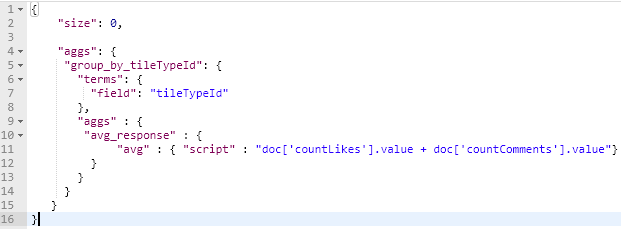
\includegraphics{script1}
	\caption{Body script 1}
	\label{fig:script1}
\end{figure}

Als we het script uitvoeren krijgen we een resultaat zoals te zien in figuur \ref{fig:scriptresult1}. Elk resultaat begint met wat algemene informatie zoals: hoeveel tijd de query nodig had, hoeveel shards er succesvol overlopen zijn, hoeveel shards faalden, hoeveel documents er voldoen aan de zoekopdracht, etc. In figuur \ref{fig:scriptresult1} is echter enkel het deel te zien dat op dit moment interessant is, namelijk de resultaten van de aggregaties.

\begin{figure}
	\centering
	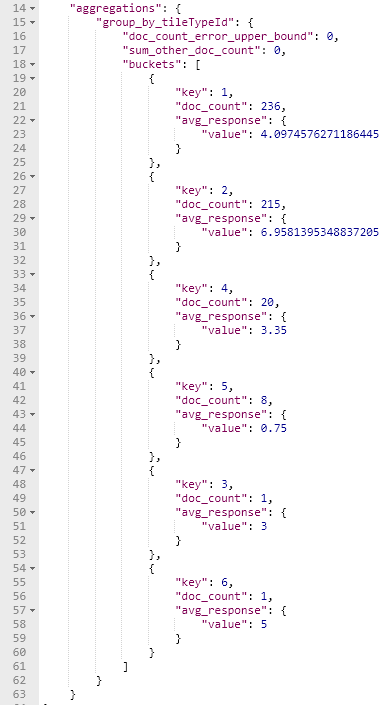
\includegraphics{scriptresult1}
	\caption{Resultaat script 1}
	\label{fig:scriptresult1}
\end{figure}

Het key-veld in de resultaten stelt telkens het tiletypeid voor waarop we groepeerden. Per aggregatie werd er een nieuwe aggregatie uitgevoerd die de gemiddelde activiteit berekende. De gemiddelde activiteit valt af te lezen in het value-veld. Het is duidelijk dat, in deze dataset, tiles met tiletypeid 2 meer activiteit vertonen dan andere tiles. Dat is leuk om te weten maar zegt op zich niet veel. We willen graag weten met welk tiletype deze id overeen komt. We stoten echter op een probleem.

Om een zoekopdracht uit te voeren op meerdere indices tegelijk zouden we de indeces bij bepaalde voorwaarden moeten samenvoegen. In SQL Server kan men dit realiseren met het JOIN-sleutelwoord. Join-operaties zijn zeer duur in Elasticsearch. Zo duur dat de ontwikkelaars ervoor zorgden dat join-operaties over verschillende indices onmogelijk zijn. Een document moet alle informatie bevatten die nodig is om te beslissen of het al dan niet in de zoekresultaten terechtkomt. Je moet dus op voorhand beslissen hoe je gaat zoeken en uw index daaraan aanpassen. Indien de query herhaaldelijk moet worden uitgevoerd vormt dat geen probleem. Maar in ons geval willen we een éénmalig antwoord op onze vraag. Dat wil zeggen dat we telkens een nieuwe index moet aanmaken en de data opnieuw importeren om er nadien slecht één query op uit te voeren. Die manier van werken zorgt voor een index overhead en beschouw ik als een groot nadeel van Elasticsearch.

Bij deze vraag zijn we echter enkel geïnteresseerd in één tiletype. Wat we ook kunnen doen is een tweede query uitvoeren op de tiletype-index. We geven het id mee en vragen zo het juiste tiletype op. Deze manier van werken heeft als voordeel dat we geen nieuwe index moeten aanmaken. De nadelen van deze manier van werken zijn dat je telkens meerdere queries moet uitvoeren en dat het niet altijd realistisch is om dat te doen. Wanneer we over tientallen documenten spreken dan gaat de voorkeur toch naar het aanmaken van een nieuwe index. Voor ons is dat niet van toepassing dus koos ik voor de tweede methode.

We maken een tweede query met URL: http://localhost:9200/tiletype/\textunderscore search. De body van de query is te zien in figuur \ref{fig:script2}. Er wordt simpelweg gezocht naar een document met id 2. In het resultaat (figuur \ref{fig:scriptresult2}) zien we dat we spreken over een tiletype idea.

Het antwoord op de eerste vraag luidt: Ja, tiles met tiletype idea werken beter dan andere.

\begin{figure}
	\centering
	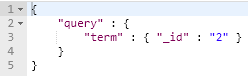
\includegraphics{script2}
	\caption{Body script 2}
	\label{fig:script2}
\end{figure}

\begin{figure}
	\centering
	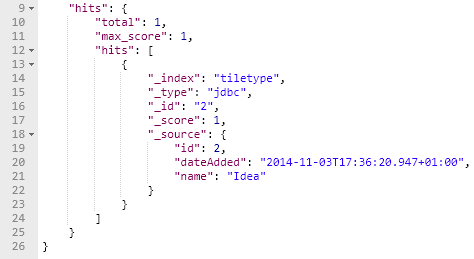
\includegraphics{scriptresult2}
	\caption{Resultaat script 2}
	\label{fig:scriptresult2}
\end{figure}

\subsubsection{Waar gebeuren de meeste likes? Vanaf de homepage of op wall pages?}
Om deze vraag te beantwoorden hebben we 3 indices nodig: like, log en logtype. Wanneer een gebruiker naar de homepage navigeert dan wordt dat gelogd in de log-tabel met logtype 8. Wanneer een gebruiker naar een wall page navigeert dan wordt dat gelogd in de log-tabel met logtype 10. Wanneer een gebruiker een tile liked dan komt er een nieuw record in de like tabel. Bij dit probleem zullen we wel verplicht zijn om een nieuwe index te maken. We willen namelijk 3 indices samennemen en we zijn geïntereseerd in alle documents.

Voor onze nieuwe index willen we de volgende structuur: de id van de like, de datum en tijd van de laatste log van de gebruiker voordat de like plaatsvond, de datum en tijd van het liken en de plaats waarop de gebruiker geliked heeft. We maken een nieuwe index aan genaamd question2 en schrijven een script om de data te importeren. Het SQL-script is te zien in figuur \ref{fig:script3}.

%% TODO: change script
\begin{figure}
	\centering
	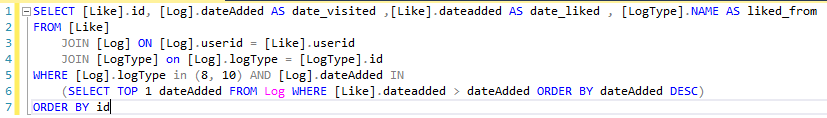
\includegraphics[width=17.5cm]{script3}
	\caption{SQL-script voor het importeren van de data uit vraag 2}
	\label{fig:script3}
\end{figure}

De index staat klaar en nu moeten we enkel nog een aggregatie doen op de plaats vanwaar er geliked werd. De URL van de query ziet er als volgt uit: http://localhost:9200/question2/\textunderscore search. In de body \textbf{TODO: figure body} geven we mee dat we een aggregatie willen op het liked\textunderscore from-veld. \textbf{TODO: result}.

\subsubsection{Heeft de lengte van de titel van een tile invloed op aantal likes}

Om het verband de tussen twee variabelen te berekenen zullen we een chi-kwadraattoets uitvoeren. \textbf{GEEF IK HIER UITLEG OVER DE CHI-KWADRAATTOETS?} Indien uit het resultaat blijkt dat er een verband is zullen we de sterkte van het verband berekenen met Cramers V. Elasticsearch biedt geen ondersteuning voor dergelijke berekeningen. Deze kunnen nochtans zeer interessant zijn bij het maken van een data-analyse. Om toch een antwoord op de vraag te krijgen zullen we Elasticsearch als hulp gebruiken bij het uitvoeren van de chi-kwadraattoets. Op die manier zal het duidelijk worden in hoeverre Elasticsearch ons kan helpen bij ingewikkelde calculaties zoals de chi-kwadraattoets en Cramers V. 

Bij het opbouwen van onze tabel gaan we zowel de lengte van de titel alsook het aantal likes opdelen in klassen. We willen een zicht krijgen van de grootte die een klasse moet krijgen. Daarom vragen we aan Elasticsearch hoelang de langste titel is en wat het grootste aantal likes is. \textbf{QUERIES} 
